\chapter{Navegación autónoma de un drone guiado por balizas visuales}\label{cap.desarrollo}
En este capítulo se describe la solución desarrollada para conseguir que un drone navegue autónomamente guiado por balizas visuales y utilizando la infraestructura mencionada anteriormente. Se explicará el diseño alto nivel de la solución y se describirá con mayor detalle las partes desarrolladas.

%\hspace{1cm} Para explicar todo los pasos primero se dara un vistazo al diseño globalmente para posteriormente explicar cada uno de los modulos indicidualmete y así poder conocer todos ellos en detalle.

\section{Diseño}
El objetivo de este proyecto es desarrollar un algoritmo para dotar a un drone de un comportamiento completamente autónomo desde el despegue, hasta el aterrizaje, ambos controlados, pasando por la localización y aproximación a diferentes posiciones 3D asociadas a las balizas, pero desconocidas de antemano. Todo esto basándose únicamente en balizas de apoyo visual. 

El componente desarrollado necesita dos ficheros de configuración. Primero un fichero xml llamado \textit{calibration.xml} que almacena los parámetros necesarios para la detección robusta de balizas arlequinadas. Segundo un fichero con la secuencia deseada de balizas AprilTags a las que se quiere que el drone visite en su navegación autónoma.

En la figura \ref{fig:Solucion final} se pueden ver las entradas y salidas de flujos de información. Adicionalmente, se han sido incluido los ficheros  imprescindibles en cada módulo para su correcto funcionamiento. Esto nos dará una imagen de alto nivel de la solución. Las comunicaciones entre procesos se llevan a cabo mediante interfaces de la biblioteca ICE. 

\begin{figure}[H]
	\begin{center}	
	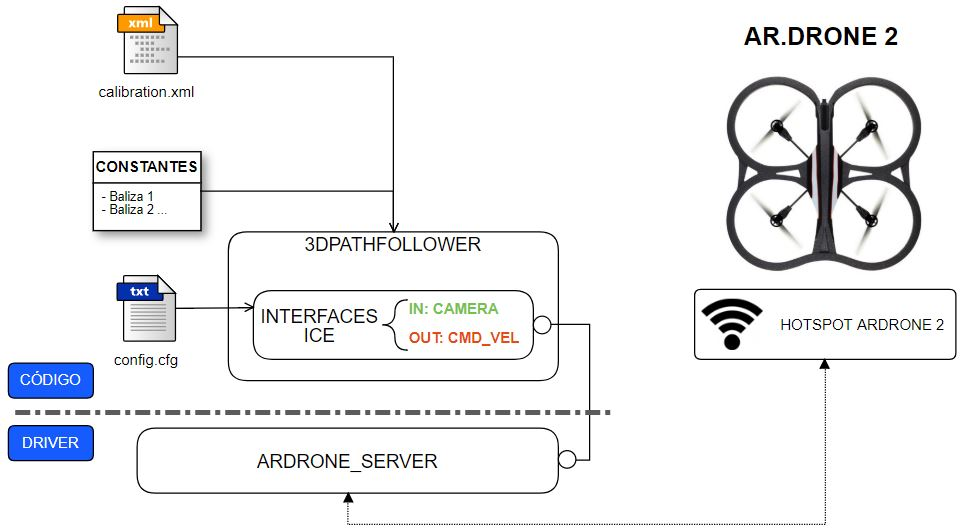
\includegraphics[scale=0.6]{imag/desgin_escenario.jpg}
	\caption{Entradas y salidas de la solución final.}
	\label{fig:Solucion final}
	\end{center}
\end{figure}

El componente 3DPahtFollower es la  aplicación mencionada anteriormente. Está compuesta por los diferentes estados del autómata, tal y como se puede apreciar en la figura \ref{fig:Solucion 3DPathFollower}. Se han agrupado los diferentes estados para una mejor comprensión del despegue controlado, navegación y búsqueda rotacional y por último, búsqueda en espiral y aterrizaje controlado. Cada uno de los estados se componen de una capa de percepción visual, que llevará a cabo la tarea de identificar las balizas y otra capa de control, que calculará y generará el comportamiento que se enviará al drone a través de las interfaces ICE. La navegación autónoma del drone se entiende aquí como la visita en secuencia a una serie de balizas AprilTags que están situadas en posiciones desconocidas por el drone, pero cercanas cada una a la siguiente en la secuencia.

\begin{figure}[H]
	\begin{center}	
		\includegraphics[scale=0.6]{imag/design_pathfollower.png}
		\caption{Diagrama de bloques del componente 3DPathFollower.}
		\label{fig:Solucion 3DPathFollower}
	\end{center}
\end{figure}

A continuación vamos a explicar cada estado y sus respectivas transiciones de las que se compone \textit{3DPathFollower} con mayor profundidad, siendo la creación de un algoritmo de navegación, el diseño de la infraestructura y la aplicación \textit{CalibrationTool} las mayores aportación de este TFG, por lo que serán los apartados en los que haremos mas hincapié. Sin embargo, al tratarse de un TFG de integración también explicaremos los módulos en los que nos hemos basado y los cambios que hemos aplicado para su correcto funcionamiento en el la aplicación final.

\section{Detección visual de las balizas}

La percepción se ha basado en la detección de dos tipos de balizas visuales: Una baliza bicolor para las fases de despegue y aterrizaje y otro tipo de balizas tipo AprilTags. 

\subsection{Balizas de aterrizaje y despegue}

Durante la realización de este TFG ha sido necesaria la configuración de filtros los de color de las balizas en los que se basa principalmente el despegue y aterrizaje controlado de la aplicación principal. Se utiliza la biblioteca de OpenCV para realizar las operaciones sobre imágenes.

Se ha escogido utilizar una baliza de color arlequinada \ref{fig:baliza arlequinada} compuesta por cuatro cuadrantes y 2 colores lo más distantes posibles en el espacio de color HSV (como por ejemplo naranja y verde), colocados de forma no contigua. Esto permitirá aumentar la robustez y reducir los posibles errores que se produzcan debido al ruido de otros colores en el ambiente.

\begin{figure}[H]
	\begin{center}	
		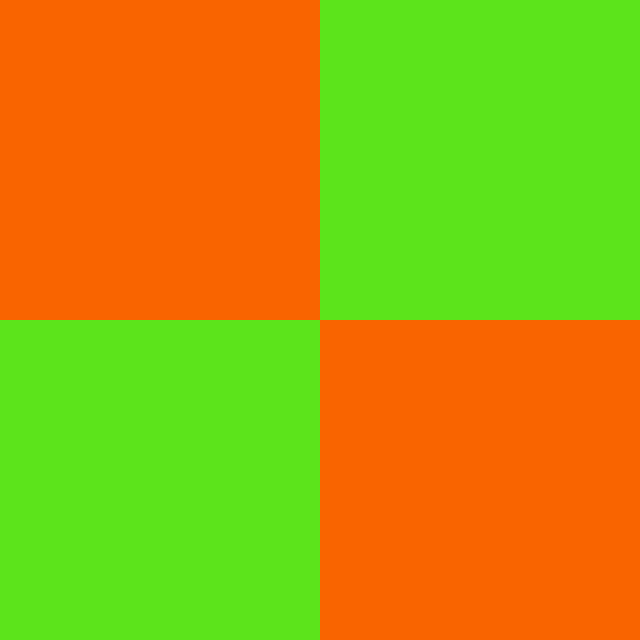
\includegraphics[scale=0.2]{imag/color_beacon_3.png}
		\caption{Ejemplo de baliza de color arlequinada.}
		\label{fig:baliza arlequinada}
	\end{center}
\end{figure}

\textit{3DPathFollower} utiliza la suma de dos filtros de color, llamados \textit{Primary} y \textit{Secondary} los diferentes valores máximos y mínimos de los componentes HSV y de las transformaciones morfológicas sobre las imágenes filtradas que explicaremos a continuación. Estas transformaciones  son la erosión y dilatación. La combinación de estas técnicas permite la eliminación de impurezas y el suavizado de la imagen, dotando de mayor robustez al filtro de color.

Se aplicará el procesado para cada uno de los dos colores, llamando a la función hsvFilter (importada de Color Tuner) y acto seguido se realizarán las transformaciones morfológicas a la imagen filtrada en HSV:

\begin{lstlisting}[backgroundcolor=\color{gray!15}]
Pmask, PmaskHSV = hsvFilter(PH_max,PS_max,PV_max,
PH_min,PS_min,PV_min,image,hsv)
PmaskHSV = cv2.erode(PmaskHSV,kernel,iterations = PErode)
PmaskHSV = cv2.dilate(PmaskHSV,kernel,iterations = PDilate)
\end{lstlisting}

Donde \textit{kernel} es el tamaño de píxeles al que se aplicará y \textit{iterations} se corresponde con la intensidad.
El resultado consistirá en la suma de ambas imágenes filtradas:
\begin{lstlisting}[backgroundcolor=\color{gray!15}]
filterImage = PmaskHSV+SmaskHSV
\end{lstlisting}

\subsection{Balizas de autolocalización}

Para la identificación de las balizas, tanto durante la búsqueda como la aproximación, se utilizarán las funciones nativas de AprilTags. Necesitaremos crear un detector para nuestra familia (36H11 \ref{FIG:34_apriltag_families}), para más adelante aplicarlo sobre una imagen convertida a escala de grises:

\begin{lstlisting}[backgroundcolor=\color{gray!15}]
self.options = apriltag.DetectorOptions()
self.detector = apriltag.Detector(self.options)
detections = self.interfaces.detector.detect(gray)
\end{lstlisting}

Para obtener esta estimación hemos tomado como referencia el algoritmo utilizado por la aplicación Slam\_Markers \ref{subsec:slam Markers} y lo hemos implementado en el lenguaje Python.

El algoritmo para estimar la posición relativa en 3D a partir de una imagen en 2D, serie de transformaciones y cálculo de matrices que a partir de las cuatro esquinas detectadas por AprilTags obtiene el vector basado en las coordenadas X,Y,Z:

\begin{lstlisting}[backgroundcolor=\color{gray!15}]
retVal,rvec,tvec =cv2.solvePnP(self.interfaces.m_MarkerPoints
,detection.corners
,self.interfaces.cameraMatrix
,self.interfaces.distCoeffs)
rodri = cv2.Rodrigues(rvec)
#We get X,Y and Z
cameraPosition = -np.matrix(rodri[0]).T * np.matrix(tvec) 
self.interfaces.x = cameraPosition.item(0)
self.interfaces.y = cameraPosition.item(1)
self.interfaces.z = cameraPosition.item(2)
\end{lstlisting}

Para calcular conocer la rotación relativa de nuestro drone con respecto a la posición baliza, se realiza una serie de transformaciones que se basan en los ángulos de euler:

\begin{lstlisting}[backgroundcolor=\color{gray!15}]
#We get roll, pitch and yaw from Euler Angles        
eulerAngles = 
self.interfaces.rotationMatrixToEulerAngles(rodri[0])
\end{lstlisting}

\section{Autómata de navegación} 
\label{sec:3Dpathfollow}
Este componente está formado por un algoritmo de navegación autónoma basado en un control representado por un autómata de estados finito. Ha sido realizado con la herramienta \textsc{Visual States}, la cuál nos ha permitido tanto desarrollar el código, como la integración con las diferentes bibliotecas y partes del sistema en un solo programa.

\begin{figure}[H]
	\begin{center}
		\includegraphics[width=0.85\textwidth]{imag/EstadosVisualStates.png}
		\caption{Estados de la aplicación 3DPathFollower}
		\label{fig: EstadosVisualStates.}	
	\end{center}
\end{figure}

En la figura \ref{fig: EstadosVisualStates.} se observan los diferentes estados y transiciones que forman la aplicación. El primer estado es el de \textit{Take-off}, en el que se envía un comando al drone para iniciar los motores en modo despegue para ganar altura y despegarse del suelo. Dado que esta fase tiene una duración de unos 2 segundos, el siguiente estado es el de \textit{Initializatión} en el que, junto a otras tareas de inicialización, se realiza la lectura del archivo de configuración \textit{calibration.xml} mostrado en la Figura \ref{fig:Solucion 3DPathFollower}, del que obtendremos los parámetros para el filtro de color. \textit{Color Beacon Tracking} se encargará de mantener estable y de forma contralada al drone encima de la baliza de color. Transcurridos 4 segundos en el objetivo, damos por estable el despegue y procedemos al estado \textit{AprilTag Rotational Search}, en el que el drone buscará mientras rota sobre sí mismo la baliza AprilTag que actualmente se considera el objetivo. Tras encontrarla pasamos a \textit{April Beacon Tracking}, el cual navegará y se situará a una distancia predeterminada durante 8 segundos, dando por satisfactoria la navegación y marcando como activa la siguiente baliza almacenada en memoria. Una vez finalizada la lista de balizas AprilTags, se activa el estado \textit{Spiral Search}, que realizará un movimiento en espiral con el objetivo de buscar nuestra baliza de aterrizaje. Si ha sido encontrada, entra en acción el estado \textit{Color Beacon Landing}, que se encargará de aterrizar de forma controlada, es decir, alineado encima de la baliza durante segundos. Tanto en \textit{April Beacon Tracking} como en  \textit{Color Beacon Landing}, en el momento en el que se pierda el campo de visión con el objetivo, se volverá al estado de búsqueda respectivo. Por último, \textit{Land} envía el comando de aterrizaje al drone y así dar por finalizado el ejercicio.



\subsection{Estado de despegue controlado}
\label{subsec:algoritmo despegue}

Este componente se basa en el TFG de Jorge Vela \cite{JorgeVela}, el cual se ha refactorizado y acoplado dentro del estado \textit{Color Beacon Tracking} en \textsc{Visual States}. Este estado se inicia una vez hemos enviado al motor la orden de iniciar el despegue e inicializado los parámetros de configuración para las balizas de color. En este estado se emplea un procesado de la imagen y un PID (Proporcional, Integral y Derivativo) (a diferencia del PD empleado originalmente por Jorge Vela), una detección de bandas muertas y un limitador de velocidad como medidas de control. 

Estableceremos como necesaria la condición de que el drone debe despegar encima de una baliza arlequinada \ref*{fig:baliza arlequinada} para comenzar el comportamiento satisfactoriamente. Por lo tanto, debemos asegurarnos de que la cámara ventral del drone esté activa y no la frontal para evitar comportamientos no deseados.

Una vez obtenemos la imagen resultante filtrada, se aplica un procesado para encontrar la cruceta que forman los cuadrantes de la baliza y encontrar así el punto central que será nuestro objetivo.

La incorporación de un PID  se debe a que el comportamiento no era lo suficientemente ágil con un PD  y se ha refactorizado y reimplementado esta parte. Ésta función de PID se aplicará en todos los algoritmos en los que este tipo de control sea necesario:

\begin{lstlisting}[backgroundcolor=\color{gray!15}]
#Proporcional
vp = kp * error
#Derivada
vd = kd * ((error-pError)/cycle)
#Integral 
viModified = ki * (vi+(error*cycle))
#Total
result = vp + vd + viModified
return  result, viModified
\end{lstlisting}

El desarrollo de este PID se ha basado en la siguiente fórmula matemática que lo describe:

\[PID(t) = (P(t) + I(t) + D(t))\]
\[P(t) = K_{p}e(t);\hspace{0.5cm}I(t) = K_{i}\int e(t) dt;\hspace{0.5cm}D(t) = K_{d}\dfrac{{de(t)}}{dt}\]

\subsection{Estados de navegación guiada por balizas}

Con el drone estable ya en el aire, el siguiente paso es cambiar a la cámara delantera y ejecutar una búsqueda rotacional y aproximación a las diferentes balizas de tipo AprilTags \ref{sec:AprilTags}. La posición de las balizas es desconocida y el orden viene dado por una lista  con los identificadores de las balizas predefinida en la sección de constantes globales de \textsc{Visual States} \ref{fig:Solucion 3DPathFollower}.

El estado de búsqueda rotacional iniciará un movimiento de giro en el sentido a las agujas del reloj y continuará girando hasta que encuentre la baliza que tiene como objetivo.
Una vez encontrado y mientras que el objetivo no se escape del campo de visión de la cámara, se ejecutará el estado de aproximación. Éste mantendrá la baliza objetivo a una altura y posición relativa centradas y una distancia preconfigurada. Para ello, necesitaremos estimar la posición relativa de la cámara del drone con respecto a la baliza en tres dimensiones. 

Una vez tenemos las estimaciones de las coordenadas y nuestra rotación con respecto a la baliza, aplicaremos un control PID, banda muerta y límites de velocidad para corregir la altura, distancia y rotación con respecto a la baliza. Este sería el código para cada una de estas componentes:

\begin{lstlisting}[backgroundcolor=\color{gray!15}]
error_xy = [self.interfaces.center[0]-self.interfaces.x,
             self.interfaces.center[1]-self.interfaces.y]
#VX
if(abs(error_xy[0])<self.interfaces.dead_band_x):
	vx=0
else:
	vx,vxiMod = self.interfaces.getPIDSpeed(error_xy[0]
	,self.interfaces.error_xy_anterior[0]
	,self.interfaces.vxi
	,self.interfaces.cycle
	,self.interfaces.kp
	,self.interfaces.kd
	,self.interfaces.ki)
	self.interfaces.vxi=vxiMod	
vx=self.interfaces.limitSpeed(vx)	
\end{lstlisting}

Para finalizar, enviaremos las velocidades combinadas a los motores para corregir al mismo tiempo las tres componentes y conseguir un comportamiento ágil y fluido. Una vez nos encontramos delante del objetivo durante más de ocho segundos, pasaremos a buscar al siguiente identificador que haya en la lista, hasta que lleguemos al final y pasemos al siguiente algoritmo.

\subsection{Estados de aterrizaje}

Para finalizar, se cambia de nuevo a la cámara ventral para dar paso a los tres últimos estados que componen el aterrizaje: \textit{Spiral Search}, \textit{Color Beacon Landing} y \textit{Land}. 
El estado \textit{Spiral Search} se corresponde con la búsqueda previa al aterrizaje controlado, para así asegurar que se encontrará de forma autónoma la baliza arlequinada. El drone describirá un movimiento en espiral, ampliando el radio de giro en función del periodo que establezcamos, hasta que encuentre la baliza:

\begin{lstlisting}[backgroundcolor=\color{gray!15}]
if(self.interfaces.cycleCounter>self.interfaces.cyclePeriod):
    self.interfaces.cycleCounter=0
    self.interfaces.xSearchSpeed+=self.interfaces.searchIncrement
xSpeed=-self.interfaces.xSearchSpeed
wSpeed=self.interfaces.wSearchSpeed        
self.interfaces.cycleCounter+=1
\end{lstlisting}

En cuanto la baliza sea detectada y mientras no se pierda el contacto visual con la baliza, se cambiará de estado para fijar la baliza en el centro del drone, aplicando las mismas técnicas que en el \textit{Algoritmo de Despegue} \ref{subsec:algoritmo despegue}. Una vez encontremos la cruceta y permanezcamos durante más de cuatro segundos en el objetivo, se activará el siguiente estado. 
En último lugar, procederemos a ejecutar el estado de \textit{Land} que enviará la señal al drone de que se debe realizar un aterrizaje. El drone aterrizará y detendrá los motores al llegar al suelo.  

\section{Configuración}

A continuación se describirá y se mostrará las configuraciones necesarias para la ejecución correcta de la aplicación.

\subsection{Configuración de la percepción}

El fichero de configuración (\textit{calibration.xml}) que aparece en la Figura \ref{fig:Solucion final}, que la herramienta calibrationTool genera para obtener los valores de las transformaciones y filtros de color que se utilizarán para la percepción de balizas arlequinadas.

\begin{lstlisting} [backgroundcolor=\color{gray!15}]
<data>
	<colour name="Primary">
		<Hmax>135</Hmax>
		<Hmin>97</Hmin>
		<Smax>255</Smax>
		<Smin>101</Smin>
		<Vmax>255</Vmax>
		<Vmin>186</Vmin>
		<Erosion>4</Erosion>
		<Dilation>4</Dilation>
	</colour>
	<colour name="Secondary">
		<Hmax>172</Hmax>
		<Hmin>150</Hmin>
		<Smax>199</Smax>
		<Smin>69</Smin>
		<Vmax>255</Vmax>
		<Vmin>0</Vmin>
		<Erosion>8</Erosion>
		<Dilation>8</Dilation>
	</colour>
</data>
\end{lstlisting}

\subsection{Configuración de interfaces}

La Figura \ref{fig:Config File} muestra el fichero de configuración (\textit{config.cfg}) de las interfaces ICE que aparece en la Figura \ref{fig:Solucion final}, que la herramienta genera para realizar las comunicaciones necesarias con el drone.

\begin{figure}[H]
	\begin{center}
		\includegraphics[width=1\textwidth]{imag/configFile.png}
		\caption{Fichero de configuración de interfaces ICE.}
		\label{fig:Config File}	
	\end{center}
\end{figure}

\subsection{Configuración de la secuencia de balizas}

Se realizará a través de la herramienta \texttt{Visual States}, en concreto, en la sección de variables globales. Se ha creado una lista con el nombre \textit{beacons} que contiene los números de los identificadores de las balizas AprilTags que queramos detectar y navegar:

\begin{lstlisting}[backgroundcolor=\color{gray!15}]
self.beacons = [4,7,16,30]
\end{lstlisting}

\section{Herramienta CalibrationTool} \label{sec:calibrationtool}

Para facilitar la tarea de calibración, nos hemos basado en la aplicación \textit{Color Tuner} \ref{subsec:colorTuner} de JdeRobot para aplicar los filtros a la imagen y la hemos enriquecido con un par de funcionalidades. Dado que \textit{3DPathFollower} utiliza la suma de dos filtros de color, llamados \textit{Primary} y \textit{Secondary}, la principal funcionalidad añadida de este herramienta es permitir la modificación simultánea de ambos filtros de color de manera que podremos visualizar al mismo tiempo la suma de las dos imágenes filtradas en la ventana \textit{Filtered\_image}. La modificación de estos filtros se realizará a través de deslizadores o \textit{sliders} tal y como se puede apreciar en la figura \ref{fig:Ejemplo CalibrationTool}.

La segunda funcionalidad añadida es la capacidad de generar o leer de un fichero de configuración en formato XML, que contendrá los diferentes valores máximos y mínimos de los componentes HSV y de las transformaciones morfológicas sobre las imágenes filtradas que explicaremos a continuación. Estas transformaciones  son la erosión y dilatación. La combinación de estas técnicas permite la eliminación de impurezas y el suavizado de la imagen, dotando de mayor robustez al filtro de color.

La adquisición se realiza a través de la interfaz de cámara ICE que contiene el fichero de configuración \textit{calib\_config.cfg} \ref{fig:Solucion final}. Para poder procesar la imagen primero es necesario verificar si ya existe un archivo de calibración (\textit{calibration.xml}) o crearlo con valores por defecto en caso negativo. Se leerán los datos del fichero de calibración  y una vez finalizados los cambios que queramos efectuar, pulsando la tecla \textit{Escape} del teclado cerrará la aplicación y generará o modificará el fichero de configuración.

En cuanto a la interfaz de usuario, para la creación de los \textit{sliders} se ha utilizado la función \textit{createTrackbar} de OpenCV:
\begin{lstlisting}[backgroundcolor=\color{gray!15}]
cv2.createTrackbar('PH_max','filtered_image',0,180,nothing)
cv2.createTrackbar('PS_max','filtered_image',0,255,nothing)
cv2.createTrackbar('PV_max','filtered_image',0,255,nothing)
cv2.createTrackbar('PH_min','filtered_image',0,255,nothing)
cv2.createTrackbar('PS_min','filtered_image',0,255,nothing)
cv2.createTrackbar('PV_min','filtered_image',0,255,nothing)
cv2.createTrackbar('PErode','filtered_image',0,100,nothing)
cv2.createTrackbar('PDilate','filtered_image',0,100,nothing)
\end{lstlisting}

Para mostrar las imágenes en pantalla se ha utilizado la función \textit{imshow} que mostrará la imagen deseada como muestra el siguiente ejemplo:

\begin{lstlisting}[backgroundcolor=\color{gray!15}]
cv2.imshow("filtered_image", filtered_image)
\end{lstlisting}


\begin{figure}[H]
	\begin{center}	
		\includegraphics[scale=0.6]{imag/calibrationTool.png}
		\caption{Ejemplo del componente CalibrationTool.}
		\label{fig:Ejemplo CalibrationTool}
	\end{center}
\end{figure}